\documentclass[11pt,a4paper]{article}

\usepackage[utf8]{inputenc}
\usepackage[T1]{fontenc}
\usepackage{lmodern}
\usepackage[margin=1in]{geometry}
\usepackage{graphicx}
\usepackage{amsmath,amssymb}
\usepackage{booktabs}
\usepackage{tabularx}
\usepackage{array}
\usepackage{float}
\usepackage{caption}
\usepackage{subcaption}
\usepackage{enumitem}
\usepackage{fancyhdr}
\usepackage{tikz}
\usetikzlibrary{arrows.meta, positioning, fit, backgrounds, calc}
\usepackage[hidelinks]{hyperref}

\graphicspath{{./figures/}{../artifacts/}{../data/captured_frames/}}

\pagestyle{fancy}
\fancyhf{}
\fancyhead[L]{\small\textit{Vision-Guided Dual-Color Robotic Sorting System (xArm 1S)}}
\fancyhead[R]{\small\textit{Sem-5 Mini-Project Report}}
\fancyfoot[C]{\small\thepage}
\renewcommand{\headrulewidth}{0.4pt}
\renewcommand{\footrulewidth}{0pt}

\setlength{\parskip}{0.45em}
\setlength{\parindent}{0pt}
\setlength{\headheight}{14pt}
\emergencystretch=2em

\begin{document}

% ----------------------------------------------------------------------------
% TITLE PAGE
% ----------------------------------------------------------------------------
\begin{titlepage}
  \centering
  \vspace*{1.2cm}
  {\large\textsc{Semester 5 Mini-Project Technical Report}\par}
  \vspace{0.8cm}
  \rule{\linewidth}{0.8pt}\\[0.5cm]
  {\LARGE\bfseries Autonomous Vision-Guided Dual-Color Robotic Sorting System Using a Single xArm 1S Manipulator\par}
  \vspace{0.4cm}
  \rule{\linewidth}{0.8pt}

  \vspace{1.2cm}
  {\large
  Design, Kinematics, Planar Homography Perception, Low-Level Bus-Servo Control,\\
  and Experimental Evaluation on Physical Hardware\par}

  \vspace{2.2cm}
  \textbf{Submitted By}\\[0.5cm]
  {\large
  Shubham Jain\\[0.2cm]
  Karan Pal\par}

  \vspace{2.5cm}
  \begin{tabular}{@{}ll@{}}
    \textbf{Manipulator Platform:} & Hiwonder / LewanSoul xArm 1S (6-DoF LX-15D Bus Servos) \\
    \textbf{Vision Sensor:}        & Logitech Webcam C270 (USB V4L2, Overhead Monocular) \\
    \textbf{Software Environment:} & Python 3, OpenCV 4.x, ROS 2 Humble (Docker), RViz2 \\
  \end{tabular}

  \vfill
  {\normalsize November 2026\par}
\end{titlepage}

% ----------------------------------------------------------------------------
% ABSTRACT
% ----------------------------------------------------------------------------
\begin{abstract}
\noindent
This report presents the mechanical setup, mathematical modeling, software architecture, and hardware validation of an autonomous dual-color sorting workcell based on a single 6-degree-of-freedom (6-DoF) Hiwonder / LewanSoul xArm~1S manipulator and an overhead Logitech C270 USB camera. Red and green craft blocks placed on a $7 \times 12$ ($350\text{ mm} \times 600\text{ mm}$) grid board are localized in metric world coordinates using four coplanar \texttt{DICT\_4X4\_50} ArUco markers and planar homography. To ensure collision-free picking and reliable sorting on low-cost bus-servo hardware, the system incorporates four primary mechanisms: (i)~multi-frame spatial consensus clustering paired with \texttt{cv2.solvePnP} 3D parallax correction; (ii)~explicit exclusion of blue HSV segmentation and spatial masking of the anodized blue robot chassis; (iii)~closed-form analytical cylindrical inverse kinematics with distance-scaled gravity sag compensation and dual-regime wrist roll alignment; and (iv)~closed-loop Motor~1 potentiometer readback over USB HID (\texttt{/dev/hidraw0}) for grasp confirmation, micro-trimming, and post-lift slip detection. Each picked block is transferred via a 7-phase overhead rear-flip trajectory to designated red and green sorting zones behind the manipulator. Across three recorded hardware trials spanning overhead, side-view, and digital-twin-synchronized runs, the system cleanly sorted 15 out of 15 blocks (100\% completion, 4-frame consensus repeatability $\sigma \le 0.37\text{ mm}$) with zero dropped objects or neighboring-block collisions, alongside 43/43 passing offline verification tests.
\end{abstract}

\newpage
\tableofcontents
\listoffigures
\listoftables
\newpage

% ============================================================================
% SECTION 1: INTRODUCTION & WORKSPACE GEOMETRY
% ============================================================================
\section{Introduction and System Overview}

\subsection{Motivation and Problem Statement}
Desktop articulated robotic arms such as the Hiwonder / LewanSoul xArm~1S provide an accessible platform for studying vision-guided manipulation, yet they exhibit physical limitations absent in industrial manipulators. Specifically, the LX-15D bus servos possess a finite $240^\circ$ mechanical travel range, plastic/brass spur gearboxes introduce $1^\circ\text{--}3^\circ$ of backlash, cantilevered link weight causes vertical tip droop at extended radial reaches, and the gripper lacks tactile force or optical contact sensors. Moreover, because the xArm~1S structural brackets are anodized blue aluminum, standard color segmentation can easily generate false object detections on the arm itself.

The objective of this project is to design and validate a complete perception-to-action pipeline that overcomes these hardware constraints using classical computer vision, analytical kinematics, and closed-loop servo feedback.

\subsection{Workspace Layout and Global Coordinate Frame}
The physical workcell is constructed on a flat $350.0\text{ mm} \times 600.0\text{ mm} \times 18.0\text{ mm}$ wooden baseboard marked with a hand-drawn $7 \times 12$ grid of $50.0\text{ mm} \times 50.0\text{ mm}$ cells. A right-handed global coordinate frame is established as follows:
\begin{itemize}[noitemsep]
  \item \textbf{Origin $(0, 0, 0)$:} Front-left corner of the baseboard (Row~11, Column~0) on the top table plane ($Z = 0.0\text{ mm}$).
  \item \textbf{$+X$ Axis:} Left to right across Columns~$0\text{--}6$ ($0.0\text{--}350.0\text{ mm}$), with the workspace midline at $X = 175.0\text{ mm}$.
  \item \textbf{$+Y$ Axis:} Front to rear across Rows~$11\text{--}0$ ($0.0\text{--}600.0\text{ mm}$).
  \item \textbf{$+Z$ Axis:} Vertically upward normal to the baseboard surface.
\end{itemize}

The manipulator is mounted centrally at $(X = 175.0\text{ mm}, Y = 375.0\text{ mm}, Z = 5.0\text{ mm})$ spanning Rows~$3\text{--}5$ and Columns~$2\text{--}4$, oriented with a nominal heading of $-90.0^\circ$ (pointing toward the front picking arena along Column~3). Table~\ref{tab:zones} summarizes the spatial layout of the workcell.

\begin{table}[H]
  \centering
  \small
  \caption{Spatial Zones and Coordinate Definitions in the Workcell}
  \label{tab:zones}
  \begin{tabularx}{\textwidth}{@{}>{\raggedright\arraybackslash}p{3.0cm} >{\raggedright\arraybackslash}p{2.6cm} >{\raggedright\arraybackslash}p{3.6cm} X@{}}
    \toprule
    \textbf{Zone / Element} & \textbf{Grid Location} & \textbf{World Coordinates (mm)} & \textbf{Role in Operation} \\
    \midrule
    xArm~1S Base Mount & Rows 3--5, Cols 2--4 & Center $(175.0, 375.0, 5.0)$ & Central mount facing $-90.0^\circ$; excluded in vision mask. \\
    Active Picking Arena & Rows 6--11, Cols 0--6 & $X \in [25, 325]$, $Y \in [25, 275]$ & Bounded by 4 ArUco markers; rectified to $600 \times 500\text{ px}$ ($2.0\text{ px/mm}$). \\
    Central Pickup Zone & Rows 7--9, Cols 2--4 & $X \in [75, 275]$, $Y \in [100, 250]$ & Primary dexterity region ($r \in [140, 260]\text{ mm}$) for plunge grasps. \\
    Red Drop Zone & Rows 0--1, Cols 0--1 & Target $(50.0, 550.0, 45.0)$ & Rear-left sorting zone ($R = 215.1\text{ mm}$); base yaw tick \texttt{650}. \\
    Green Drop Zone & Rows 0--1, Cols 5--6 & Target $(300.0, 550.0, 45.0)$ & Rear-right sorting zone ($R = 215.1\text{ mm}$); base yaw tick \texttt{354}. \\
    \bottomrule
  \end{tabularx}
\end{table}

% ============================================================================
% SECTION 2: EQUIPMENT & HARDWARE SPECIFICATIONS
% ============================================================================
\section{Equipment and Hardware Specifications}

\subsection{Workcell Hardware Components}
Table~\ref{tab:bom} lists the physical equipment used in the live sorting setup, and Figure~\ref{fig:workcell} shows the assembled testbench during operation. During live sorting trials, blocks are placed directly on the wooden grid board and deposited onto the designated rear-left (red) and rear-right (green) grid zones behind the manipulator (physical $100\times 100\times 35\text{ mm}$ collection boxes are also supported in the mechanical specification and URDF model).

\begin{table}[H]
  \centering
  \small
  \caption{Hardware and Equipment Used in the Sorting Workcell}
  \label{tab:bom}
  \begin{tabularx}{\textwidth}{@{}>{\raggedright\arraybackslash}p{2.4cm} >{\raggedright\arraybackslash}p{3.3cm} >{\raggedright\arraybackslash}p{4.0cm} X@{}}
    \toprule
    \textbf{Subsystem} & \textbf{Equipment} & \textbf{Specification} & \textbf{Function} \\
    \midrule
    Manipulator & Hiwonder / LewanSoul xArm~1S & 6-DoF articulated arm, 6$\times$ LX-15D bus servos, blue aluminum chassis & Executes picking, vertical lift, overhead rear-flip, and release. \\
    End-Effector & 2-Finger Parallel Claw & $0\text{--}55\text{ mm}$ jaw span, axial wrist roll (M2) + clamp (M1) & Grasps craft blocks along aligned square or rectangular faces. \\
    Overhead Camera & Logitech Webcam C270 & USB UVC (\texttt{046d:0825}), Linux V4L2 (\texttt{/dev/video*}) & Captures overhead frames for ArUco calibration and HSV segmentation. \\
    Lighting & 10" LED Ring Light & USB-powered dimmable ring light on adjustable tripod stand & Provides diffuse workspace illumination to stabilize HSV thresholds. \\
    Base Platform & Wooden Grid Board & $350 \times 600 \times 18\text{ mm}$ board with hand-drawn $7 \times 12$ ($5\text{ cm}$) grid & Flat $Z=0$ work surface; xArm rests on $5\text{ mm}$ spacer plate. \\
    Fiducials & 4$\times$ Printed ArUco Markers & \texttt{DICT\_4X4\_50} (IDs 0--3), $50 \times 50\text{ mm}$, flat on board & Defines metric planar homography ($2.0\text{ px/mm}$) and 3D pose. \\
    Target Objects & Painted Craft Blocks & Matte red and green wooden blocks ($37.5 \times 37.5 \times 45.0\text{ mm}$ nominal) & Sorted by color into left and right rear drop zones. \\
    Power Supply & Regulated DC Adapter & $7.4\text{ V} / 5\text{ A}$ DC supply & Supplies peak servo current to the xArm bus without brownout. \\
    Host Computer & Ubuntu Linux Laptop & USB HID (\texttt{/dev/hidraw0}), Python \texttt{venv}, Docker ROS~2 Humble & Runs vision pipeline, IK solver, hardware driver, and digital twin. \\
    \bottomrule
  \end{tabularx}
\end{table}

\begin{figure}[H]
  \centering
  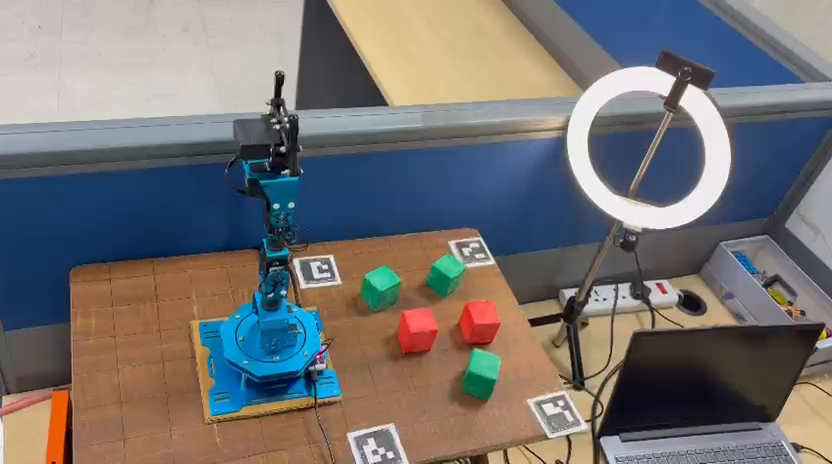
\includegraphics[width=0.72\textwidth]{workcell_setup.png}
  \caption{Assembled physical sorting workcell showing the Hiwonder xArm~1S on the $7 \times 12$ wooden grid board, four coplanar ArUco markers, five target blocks, the 10" LED ring light on stand, and the host laptop.}
  \label{fig:workcell}
\end{figure}

\subsection{Link Dimensions and Servo ID Mapping}
From calibrated measurements in \texttt{config/xarm\_hardware.yaml}, the manipulator link lengths are:
\begin{itemize}[noitemsep]
  \item Base-to-shoulder elevation: $d_1 = 70.0\text{ mm}$ ($65.0\text{ mm}$ base pillar $+ 5.0\text{ mm}$ mounting plate).
  \item Upper arm length: $L_1 = 101.0\text{ mm}$ (shoulder axis to elbow axis).
  \item Forearm length: $L_2 = 95.0\text{ mm}$ (elbow axis to wrist pitch axis).
  \item Tool length to grip pad center: $L_{3,\text{grip}} = 150.0\text{ mm}$ (outer fingertip length $L_{3,\text{tip}} = 168.0\text{ mm}$).
\end{itemize}

On the Hiwonder 1-wire half-duplex bus, servo IDs are addressed \textbf{tip-to-base} (reverse of standard Denavit--Hartenberg base-to-tip indexing). Table~\ref{tab:motors} documents the hardware ID mapping, software tick limits, and angular scale factors.

\begin{table}[H]
  \centering
  \small
  \caption{xArm 1S Servo Hardware ID Mapping, Safe Limits, and Angular Scales}
  \label{tab:motors}
  \begin{tabularx}{\textwidth}{@{}>{\centering\arraybackslash}p{1.2cm} >{\raggedright\arraybackslash}p{2.3cm} c c >{\centering\arraybackslash}p{2.0cm} X@{}}
    \toprule
    \textbf{ID} & \textbf{Joint Name} & \textbf{Safe Ticks} & \textbf{Center} & \textbf{Scale} & \textbf{Motion Convention} \\
    \midrule
    \textbf{M1} & Claw Gripper & $250\text{--}750$ & $500$ & $0\text{--}55\text{ mm}$ & $250$ open ($55\text{ mm}$); $750$ closed ($0\text{ mm}$). \\
    \textbf{M2} & Wrist Roll & $130\text{--}870$ & $500$ & $0.2432^\circ/\text{tick}$ & $130$ CW $90^\circ$; $500$ level; $870$ CCW $90^\circ$. \\
    \textbf{M3} & Wrist Pitch & $140\text{--}860$ & $500$ & $0.2400^\circ/\text{tick}$ & $500$ collinear with forearm; $860$ arena lean; $140$ rear lean. \\
    \textbf{M4} & Elbow Pitch & $140\text{--}860$ & $500$ & $0.2400^\circ/\text{tick}$ & $500$ collinear ($180^\circ$); $140$ folds forward; $860$ folds rear. \\
    \textbf{M5} & Shoulder Pitch & $140\text{--}860$ & $500$ & $0.2400^\circ/\text{tick}$ & $500$ vertical ($90^\circ$); $860$ leans forward; $140$ leans rear. \\
    \textbf{M6} & Base Yaw & $120\text{--}880$ & $500$ & $0.2368^\circ/\text{tick}$ & $500$ South ($-90^\circ$); $120$ CW $90^\circ$; $880$ CCW $90^\circ$. \\
    \bottomrule
  \end{tabularx}
\end{table}

% ============================================================================
% SECTION 3: BASIC WORKING STEPS
% ============================================================================
\section{Basic Working Steps}

The operational workflow from hardware startup to completed sorting proceeds in four sequential steps, executable via the web interface (\texttt{tools/autonomous\_dashboard.py}), the terminal pipeline (\texttt{tools/run\_autonomous\_system.py}), or ROS~2 launch files (\texttt{xarm.launch.py}):

\begin{enumerate}[leftmargin=1.6em, itemsep=0.45em]
  \item \textbf{Hardware Discovery and Device Verification:} The software scans Linux sysfs for the xArm~1S USB HID controller (\texttt{0483:5750} on \texttt{/dev/hidraw0}, with \texttt{/dev/ttyUSB*} serial fallback) and enumerates V4L2 video nodes (\texttt{/dev/video*}) to bind the external Logitech C270 camera while ignoring internal laptop cameras and metadata streams.
  \item \textbf{Camera Alignment and Multi-Frame Locking:} Using the alignment overlay, the overhead camera is positioned above the arena until all four corner ArUco markers (\texttt{DICT\_4X4\_50}) are detected and camera height/tilt checks pass. Up to four stationary frames are captured and fused via spatial consensus so the scene remains locked even if a hand-held camera is lowered during execution.
  \item \textbf{Arena Rectification and Target Queue Construction:} Each frame is undistorted, perspective-warped into a $600 \times 500\text{ px}$ metric grid ($2.0\text{ px/mm}$), masked over the arm base area, and segmented in HSV color space for red and green blocks. Valid detections are converted into arm polar coordinates $(r, \theta_{\text{arm}})$ and ordered in ascending radial distance $r$ (Nearest-First).
  \item \textbf{Closed-Loop Pick, Overhead Rear-Flip, and Placement:} For each target in the queue, analytical IK computes joint ticks for hover standoff and vertical plunge. After closed-loop potentiometer micro-trimming and Motor~1 clamp verification, the arm lifts the block vertically, flips backward over the shoulder, rotates Motor~6 to the red (\texttt{650}) or green (\texttt{354}) rear drop yaw, opens the gripper, and returns to its home pose.
\end{enumerate}

% ============================================================================
% SECTION 4: INTERNAL ARCHITECTURE & ALGORITHMS
% ============================================================================
\section{Internal Architecture and Working Principles}

Figure~\ref{fig:arch} illustrates the internal modular pipeline linking camera capture, vision processing, trajectory scheduling, low-level servo communication, and optional ROS~2 digital twin synchronization.

\begin{figure}[H]
  \centering
  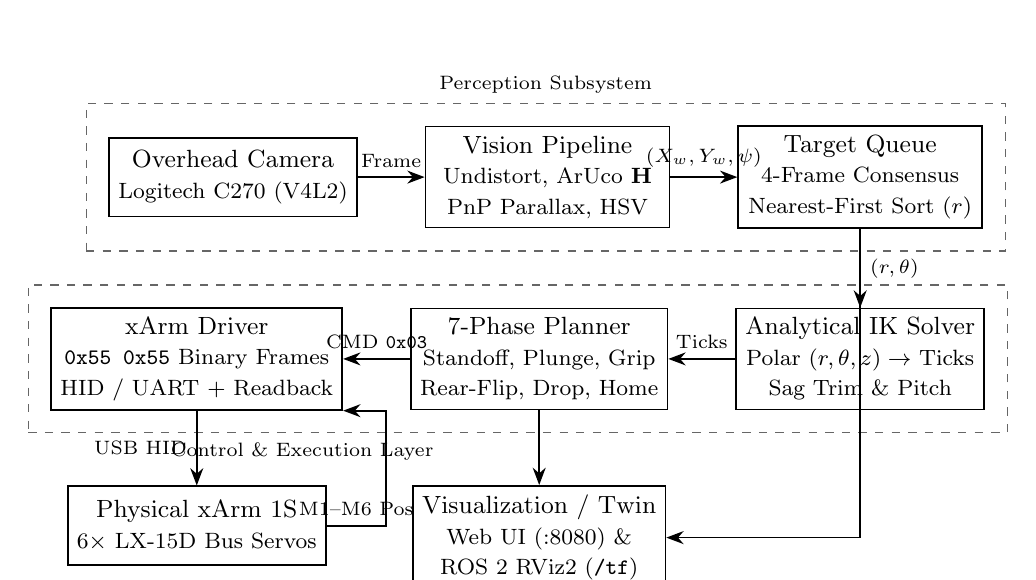
\begin{tikzpicture}[
    node distance=0.75cm and 0.85cm,
    blk/.style={draw=black, semithick, fill=white, minimum width=3.1cm, minimum height=1.0cm, align=center, font=\small},
    grp/.style={draw=black!60, dashed, inner sep=8pt},
    arr/.style={-{Stealth[length=2.2mm]}, semithick, black}
  ]
    % Top row: Perception
    \node[blk] (cam) {Overhead Camera\\{\footnotesize Logitech C270 (V4L2)}};
    \node[blk, right=of cam] (cv) {Vision Pipeline\\{\footnotesize Undistort, ArUco $\mathbf{H}$}\\{\footnotesize PnP Parallax, HSV}};
    \node[blk, right=of cv] (cons) {Target Queue\\{\footnotesize 4-Frame Consensus}\\{\footnotesize Nearest-First Sort ($r$)}};

    % Middle row: Kinematics & Control
    \node[blk, below=1.0cm of cons] (ik) {Analytical IK Solver\\{\footnotesize Polar $(r,\theta,z) \to$ Ticks}\\{\footnotesize Sag Trim \& Pitch}};
    \node[blk, left=of ik] (traj) {7-Phase Planner\\{\footnotesize Standoff, Plunge, Grip}\\{\footnotesize Rear-Flip, Drop, Home}};
    \node[blk, left=of traj] (drv) {xArm Driver\\{\footnotesize \texttt{0x55 0x55} Binary Frames}\\{\footnotesize HID / UART + Readback}};

    % Bottom row: Hardware & Twin
    \node[blk, below=0.95cm of drv] (hw) {Physical xArm 1S\\{\footnotesize 6$\times$ LX-15D Bus Servos}};
    \node[blk, below=0.95cm of traj] (twin) {Visualization / Twin\\{\footnotesize Web UI (:8080) \&}\\{\footnotesize ROS~2 RViz2 (\texttt{/tf})}};

    \begin{scope}[on background layer]
      \node[grp, fit=(cam)(cv)(cons), label={[font=\scriptsize]above:Perception Subsystem}] {};
      \node[grp, fit=(ik)(traj)(drv), label={[font=\scriptsize]below left:Control \& Execution Layer}] {};
    \end{scope}

    \draw[arr] (cam) -- node[above, font=\scriptsize]{Frame} (cv);
    \draw[arr] (cv) -- node[above, font=\scriptsize]{$(X_w,Y_w,\psi)$} (cons);
    \draw[arr] (cons) -- node[right, font=\scriptsize]{$(r,\theta)$} (ik);
    \draw[arr] (ik) -- node[above, font=\scriptsize]{Ticks} (traj);
    \draw[arr] (traj) -- node[above, font=\scriptsize]{CMD \texttt{0x03}} (drv);
    \draw[arr] (drv) -- node[left, font=\scriptsize]{USB HID} (hw);
    \draw[arr] (hw.east) -- node[above, font=\scriptsize]{M1--M6 Pos} ++(0.75,0) |- (drv.south east);
    \draw[arr] (traj) -- (twin);
    \draw[arr] (cons.south) |- (twin.east);
  \end{tikzpicture}
  \caption{Block diagram of the internal perception, planning, and hardware control pipeline.}
  \label{fig:arch}
\end{figure}

\subsection{Computer Vision and Spatial Calibration}
The vision module (\texttt{vision/arena\_vision\_pipeline.py}) processes frames using classical OpenCV operations for deterministic latency under $25\text{ ms}$:

\begin{enumerate}[leftmargin=1.5em]
  \item \textbf{Resolution-Scaled Undistortion:} Camera intrinsics $\mathbf{K}$ and distortion coefficients $\mathbf{D} = [k_1, k_2, p_1, p_2, k_3]$ stored in \texttt{config/\allowbreak camera\_\allowbreak calibration.yaml} are scaled dynamically to the active stream resolution and applied via \texttt{cv2.undistort()} prior to marker detection.
  \item \textbf{ArUco Detection and Planar Homography:} Four $50 \times 50\text{ mm}$ \texttt{DICT\_4X4\_50} markers positioned at $(25, 275)$, $(325, 275)$, $(25, 25)$, and $(325, 25)\text{ mm}$ are detected with sub-pixel corner refinement (\texttt{CORNER\_\allowbreak REFINE\_\allowbreak SUBPIX}), a $20\text{ px}$ white border pad to preserve quiet zones near frame edges, and a CLAHE contrast fallback. Perspective transformation yields a $600 \times 500\text{ px}$ rectified grid at $2.0\text{ px/mm}$:
  \begin{equation}
    X_w = 25.0 + \frac{\bar{u}}{2.0}, \qquad Y_w = 275.0 - \frac{\bar{v}}{2.0}
  \end{equation}
  \item \textbf{3D Pose and Parallax Correction:} Using \texttt{cv2.solvePnP} on the four coplanar markers, the pipeline estimates the camera position $(X_c, Y_c, H_c)$ and depression angle. Because blocks have finite height ($45.0\text{ mm}$ nominal), their upper surface projects radially outward from the camera nadir point relative to the $Z = 0$ plane. The apparent world coordinates are corrected via:
  \begin{equation}
    X_{w,\text{corr}} = X_w - (X_w - X_c)\frac{z_{\text{eff}}}{H_c}, \qquad
    Y_{w,\text{corr}} = Y_w - (Y_w - Y_c)\frac{z_{\text{eff}}}{H_c}
  \end{equation}
  where $z_{\text{eff}}$ blends between block center height ($22.5\text{ mm}$) and top-face height ($36.0\text{ mm}$) according to apparent contour area excess, and $(X_c, Y_c)$ is clamped within arena limits for near-nadir views ($\ge 80^\circ$) to suppress lateral PnP jitter.
  \item \textbf{HSV Segmentation and Chassis Exclusion:} Red blocks are segmented across dual hue bands ($H \in [0, 12] \cup [168, 180]$, $S \ge 90$, $V \ge 60$) and green blocks across $H \in [38, 96]$, $S \ge 75$, $V \ge 50$. Blue segmentation is disabled in \texttt{config/colors.yaml}, and the arm base region ($X_w \in [100, 250]\text{ mm}$, $Y_w \in [300, 450]\text{ mm}$) is masked out. After $5 \times 5$ elliptical morphological opening/closing and area/aspect filtering ($1000\text{--}25000\text{ px}^2$, $\text{AR} \le 2.5$), image moments $(M_{10}/M_{00}, M_{01}/M_{00})$ extract centroids and \texttt{cv2.minAreaRect} computes planar yaw $\psi \in [-45^\circ, +45^\circ]$.
  \item \textbf{Multi-Frame Consensus:} \texttt{build\_multiframe\_consensus\_queue()} clusters detections across up to four snapped frames within a $25\text{ mm}$ radius, discards transient detections appearing in fewer than $\lceil N/2 \rceil$ frames, and takes the median $(X_w, Y_w, Z_w)$ and median wrist roll tick.
\end{enumerate}

\subsection{Analytical Inverse Kinematics and Mechanical Compensation}
Implemented in \texttt{ros2\_ws/\allowbreak src/\allowbreak sorting\_arm/\allowbreak sorting\_arm/\allowbreak kinematics.py}, the IK solver decouples 3D positioning into base yaw rotation and planar 3-link geometry relative to the base mount $(X_b = 175.0\text{ mm}, Y_b = 375.0\text{ mm}, Z_b = 5.0\text{ mm})$ with nominal heading $\theta_{\text{nom}} = -90.0^\circ$:
\begin{equation}
  r = \sqrt{(X_w - X_b)^2 + (Y_w - Y_b)^2}, \qquad
  \theta_{\text{arm}} = \operatorname{atan2}(Y_w - Y_b, X_w - X_b) - \theta_{\text{nom}}
\end{equation}

\subsubsection*{Approach Pitch Scheduling}
A purely vertical grasp ($\phi = -90^\circ$) requires the wrist joint at $z_w = z + L_3 \approx 172.5\text{ mm}$ ($\Delta z = 102.5\text{ mm}$ above shoulder $d_1 = 70.0\text{ mm}$). With $L_1 + L_2 = 196.0\text{ mm}$, vertical picking saturates at $\sqrt{196^2 - 102.5^2} \approx 167\text{ mm}$, leaving most of the arena unreachable. To span $r \in [110, 325]\text{ mm}$, \texttt{compute\_natural\_pitch(r, z)} schedules a steep plunge ($\phi \in [-79^\circ, -72^\circ]$) for near targets ($r < 195\text{ mm}$) and transitions smoothly to shallower angles ($\phi \to -25^\circ$) at outer reaches, with an automatic $\pm 1^\circ\text{--}\pm 25^\circ$ fallback search if joint limits are reached.

\subsubsection*{Closed-Form Geometric Equations}
Given effective radial reach $r_{\text{eff}}$ and pitch $\phi$, the wrist offset relative to the shoulder pivot $(0, d_1)$ is:
\begin{equation}
  r' = r_{\text{eff}} - L_3 \cos\phi, \qquad
  z' = (z - z_{\text{trim}}) - L_3 \sin\phi - d_1, \qquad
  D = \sqrt{(r')^2 + (z')^2}
\end{equation}
Solving the two-link triangle in the Elbow-Up configuration gives the interior elbow angle $\alpha_3$ and shoulder angle $\theta_{\text{shoulder}}$:
\begin{align}
  \alpha_3 &= \arccos\!\left(\operatorname{clip}\!\left(\frac{L_1^2 + L_2^2 - D^2}{2 L_1 L_2},\, -1,\, 1\right)\right) \\
  \theta_{\text{shoulder}} &= \operatorname{atan2}(z', r') + \arccos\!\left(\operatorname{clip}\!\left(\frac{L_1^2 + D^2 - L_2^2}{2 L_1 D},\, -1,\, 1\right)\right)
\end{align}
The forearm angle is $\theta_{\text{forearm}} = \theta_{\text{shoulder}} - (180^\circ - \alpha_3)$, and the relative wrist pitch is $\theta_{\text{wrist}} = \phi - \theta_{\text{forearm}}$.

\subsubsection*{Distance-Scaled Sag Compensation and Dual-Regime Wrist Roll}
To compensate cantilever link droop and gear play at extended reaches without overshooting near targets, radial sag compensation ramps linearly over $r \in [185, 250]\text{ mm}$:
\begin{equation}
  s_{\text{sag}}(r) = \operatorname{clip}\!\left(\frac{r - 185.0}{65.0},\, 0,\, 1\right), \qquad
  r_{\text{eff}} = r + s_{\text{sag}}(r)\,\big[\delta_0 + k_{\text{reach}}\max(0,\, r - 185.0)\big]
\end{equation}
For wrist roll (Motor~2), near-field square blocks ($r < 195\text{ mm}$) rotate to align the jaws with the nearest block face, and elongated blocks ($\text{AR} \ge 1.25$) rotate $90^\circ$ ($130\text{ ticks}$) if oriented lengthwise along $X$; for far reaches ($r \ge 195\text{ mm}$), roll is locked level at $500\text{ ticks}$ so neither fingertip tilts downward into the board.

\subsection{7-Phase Overhead Rear-Flip Trajectory and Nearest-First Policy}
Target objects are sorted in ascending radial distance $r$ (Nearest-First) so inner blocks are removed before reaching outer blocks, preventing forearm collisions. Each pick-and-place cycle executes seven phases (Table~\ref{tab:phases}). Because the rear drop targets lie at base yaw ticks \texttt{650} (red) and \texttt{354} (green), Motor~6 operates solely within $[354, 650]\text{ ticks}$ ($\approx 71^\circ$ span), avoiding the $240^\circ$ LX-15D servo deadzone and cable twist.

\begin{table}[H]
  \centering
  \small
  \caption{7-Phase Overhead Rear-Flip Pick-and-Place Sequence}
  \label{tab:phases}
  \begin{tabularx}{\textwidth}{@{}>{\centering\arraybackslash}p{0.8cm} >{\raggedright\arraybackslash}p{2.7cm} >{\raggedright\arraybackslash}p{3.1cm} >{\centering\arraybackslash}p{1.8cm} X@{}}
    \toprule
    \textbf{Ph.} & \textbf{Phase Name} & \textbf{Target Pose} & \textbf{Claw (M1)} & \textbf{Internal Control \& Safety Action} \\
    \midrule
    1 & Overhead Standoff & $(r, \theta, Z = 80\text{ mm})$ & Open ($250$) & Clears $45\text{ mm}$ blocks and adjacent targets prior to descent. \\
    2 & Vertical Plunge & $(r, \theta, Z_{\text{pick}})$ & Open ($250$) & Vertical descent followed by potentiometer micro-trim ($\pm 2\text{--}12\text{ ticks}$). \\
    3 & Firm Clamping & $(r, \theta, Z_{\text{pick}})$ & Close ($750$) & Clamps block; Motor~1 readback confirms grasp ($< 650\text{ ticks}$). \\
    4 & Vertical Lift & $(r, \theta, Z = 90\text{ mm})$ & Clamp ($750$) & Lifts vertically; post-lift Motor~1 readback aborts if block slips. \\
    5 & Rear-Flip Transit & $[500, 350, 500, 450]$ & Clamp ($750$) & Pitches arm backward overhead while Motor~6 slews to target bin yaw. \\
    6 & Drop \& Release & Red: \texttt{650} / Grn: \texttt{354} & Open ($250$) & Descends to $(50/300, 550, 45)\text{ mm}$ zone and releases block. \\
    7 & Home Reset & $[500,500,500,500,500]$ & Open ($250$) & Returns to upright neutral stance before next queued object. \\
    \bottomrule
  \end{tabularx}
\end{table}

\subsection{Low-Level Communication and Closed-Loop Verification}
The hardware driver (\texttt{sorting\_arm/\allowbreak xarm\_\allowbreak protocol.py}) supports native USB HID (\texttt{/dev/hidraw*}, 65-byte reports with Report ID \texttt{0x00}) and UART serial (\texttt{/dev/ttyUSB*}). Binary command packets follow the Hiwonder frame structure:
\begin{center}
  \footnotesize\texttt{0x55 0x55 [Length] [CMD] [Count] [Time\_L] [Time\_H] [ID\_1] [Pos1\_L] [Pos1\_H] ...}
\end{center}
using \texttt{CMD\_SERVO\_MOVE = 0x03} for synchronized multi-servo moves, \texttt{CMD\_MULT\_SERVO\_UNLOAD = 0x14} for torque-off emergency stop, and \texttt{CMD\_SERVO\_POS\_READ = 0x15} for potentiometer readback. Prior to HID polling, up to $32$ stale input reports are drained from the kernel buffer to ensure current shaft readings. If Motor~1 reads $\ge 650\text{ ticks}$ after clamping (empty claw), the controller checks whether any neighbor lies within $85\text{ mm}$: if clear, one lower-altitude retry ($Z_{\text{pick}} - 2\text{ mm}$) is attempted; otherwise, the pick aborts to avoid disturbing adjacent blocks.

\subsection{Software Environments (ROS 2 Humble \& Host Dashboard)}
The codebase maintains two isolated runtime environments:
\begin{itemize}[noitemsep]
  \item \textbf{Dockerized ROS~2 Humble Workspace:} Runs \texttt{driver\_node}, \texttt{vision\_node}, \texttt{autonomous\_sorter\_node}, \texttt{arena\_visualizer\_node}, and \texttt{robot\_state\_publisher} with \texttt{urdf/xarm\_1s.urdf} in RViz2 via \texttt{./docker/run.sh}.
  \item \textbf{Host Python Virtual Environment:} Executes \texttt{tools/\allowbreak autonomous\_\allowbreak dashboard.py} (HTTP/MJPEG interface on port \texttt{8080} with optional ROS~2 topic bridging), \texttt{tools/\allowbreak web\_config/\allowbreak server.py} (servo calibration and CSV drift telemetry on port \texttt{8000}), and standalone vision utilities.
\end{itemize}

% ============================================================================
% SECTION 5: EXPERIMENTAL DEMONSTRATION & VERIFICATION RESULTS
% ============================================================================
\section{Experimental Results and Verification}

\subsection{Multi-Trial Hardware Validation Summary}
Three independent live hardware sorting runs were recorded under full autonomous execution (five blocks per trial: two red and three green), covering digital-twin telemetry capture, side-view observation under LED ring-light illumination, and overhead arena verification. Table~\ref{tab:trials} summarizes the performance across all three trials.

\begin{table}[H]
  \centering
  \small
  \caption{Summary of Recorded Live Hardware Sorting Trials}
  \label{tab:trials}
  \begin{tabularx}{\textwidth}{@{}>{\raggedright\arraybackslash}p{1.6cm} >{\raggedright\arraybackslash}p{4.3cm} c c X@{}}
    \toprule
    \textbf{Trial} & \textbf{Recording / Viewpoint} & \textbf{Duration} & \textbf{Sorted} & \textbf{Key Verified Observations} \\
    \midrule
    Trial~1 & Digital Twin + Console Log (\texttt{10.55.42 AM.mp4}) & $43.6\text{ s}$ & $5 / 5$ & Nearest-First span $192.7\text{--}292.8\text{ mm}$; consensus $\sigma \in [0.20, 0.37]\text{ mm}$; M1 grip readbacks $546\text{--}558\text{ ticks}$. \\
    Trial~2 & Side View with Ring Light (\texttt{12.34.10 PM.mp4}) & $50.7\text{ s}$ & $5 / 5$ & Clean overhead transfer under tripod LED ring light; stacked Green~\#2 atop Green~\#1 on rear zone. \\
    Trial~3 & Overhead Arena View (\texttt{12.40.06 PM.mp4}) & $42.8\text{ s}$ & $5 / 5$ & All 3 green and 2 red blocks grouped cleanly on opposite rear flanks ($\approx 8.5\text{ s}$/block). \\
    \midrule
    \textbf{Total} & \textbf{3 Independent Live Runs} & \textbf{137.1\,s} & \textbf{15 / 15} & \textbf{100\% pick-and-place success; 0 drops or neighbor collisions.} \\
    \bottomrule
  \end{tabularx}
\end{table}

\subsection{Logged Consensus Telemetry and Side-View Execution (Trials 1 \& 2)}
During Trial~1, four stationary frames were snapped prior to execution, locking all four corner ArUco markers and computing per-target 4-frame median coordinates. Table~\ref{tab:trial1_telemetry} lists the exact logged target queue and closed-loop verification values observed during execution. Note that closed-loop potentiometer micro-trimming automatically corrected up to $11\text{ ticks}$ of servo deadband during vertical plunge, and Motor~1 grip readbacks ($546$ and $558\text{ ticks}$) stayed well below the $650$-tick empty-jaw threshold both after clamping and after vertical liftoff.

\begin{table}[H]
  \centering
  \small
  \caption{Logged 4-Frame Consensus Queue and Execution Telemetry (Trial 1)}
  \label{tab:trial1_telemetry}
  \begin{tabularx}{\textwidth}{@{}c c c c c c X@{}}
    \toprule
    \textbf{\#} & \textbf{Color} & \textbf{Arena $(X, Y)$ (mm)} & \textbf{Reach $r$ (mm)} & \textbf{4-Frame $\sigma$ (mm)} & \textbf{Roll Tick} & \textbf{Drop Yaw / Logged Readback} \\
    \midrule
    1 & Green & $(258.5, 201.3)$ & $192.7$ & $0.37$ & $518$ ($+4^\circ$) & Green (\texttt{354}); trim $11\text{ ticks}$, M1 $= 557\text{ ticks}$. \\
    2 & Red   & $(177.2, 173.6)$ & $201.4$ & $0.32$ & $500$ (Level)      & Red (\texttt{650}); 4/4 frames locked. \\
    3 & Green & $(94.2, 114.2)$  & $273.1$ & $0.21$ & $500$ (Level)      & Green (\texttt{354}); 4/4 frames locked. \\
    4 & Green & $(266.8, 97.7)$  & $292.1$ & $0.25$ & $500$ (Level)      & Green (\texttt{354}); trim $11\text{ ticks}$, M1 $= 558\text{ ticks}$. \\
    5 & Red   & $(174.6, 82.2)$  & $292.8$ & $0.20$ & $500$ (Level)      & Red (\texttt{650}); trim $11\text{ ticks}$, M1 $= 546\text{ ticks}$. \\
    \bottomrule
  \end{tabularx}
\end{table}

Figure~\ref{fig:dashboard} shows the Workcell Operator Console (\texttt{localhost:8080}) captured during Trial~1 while executing Phase~2 (Plunge) on Target~\#2 after Target~\#1 had been deposited into the green drop zone. The interface displays live USB hardware health (\texttt{/dev/video4} and \texttt{hidraw3}), 4-corner ArUco lock indicators (93\% alignment quality at $H_c = 60.3\text{ cm}$ and $83.8^\circ$ tilt), the synchronized 3D Digital Twin viewport, the Nearest-First target queue, the active trajectory step indicator, and real-time servo feedback logs.

\begin{figure}[H]
  \centering
  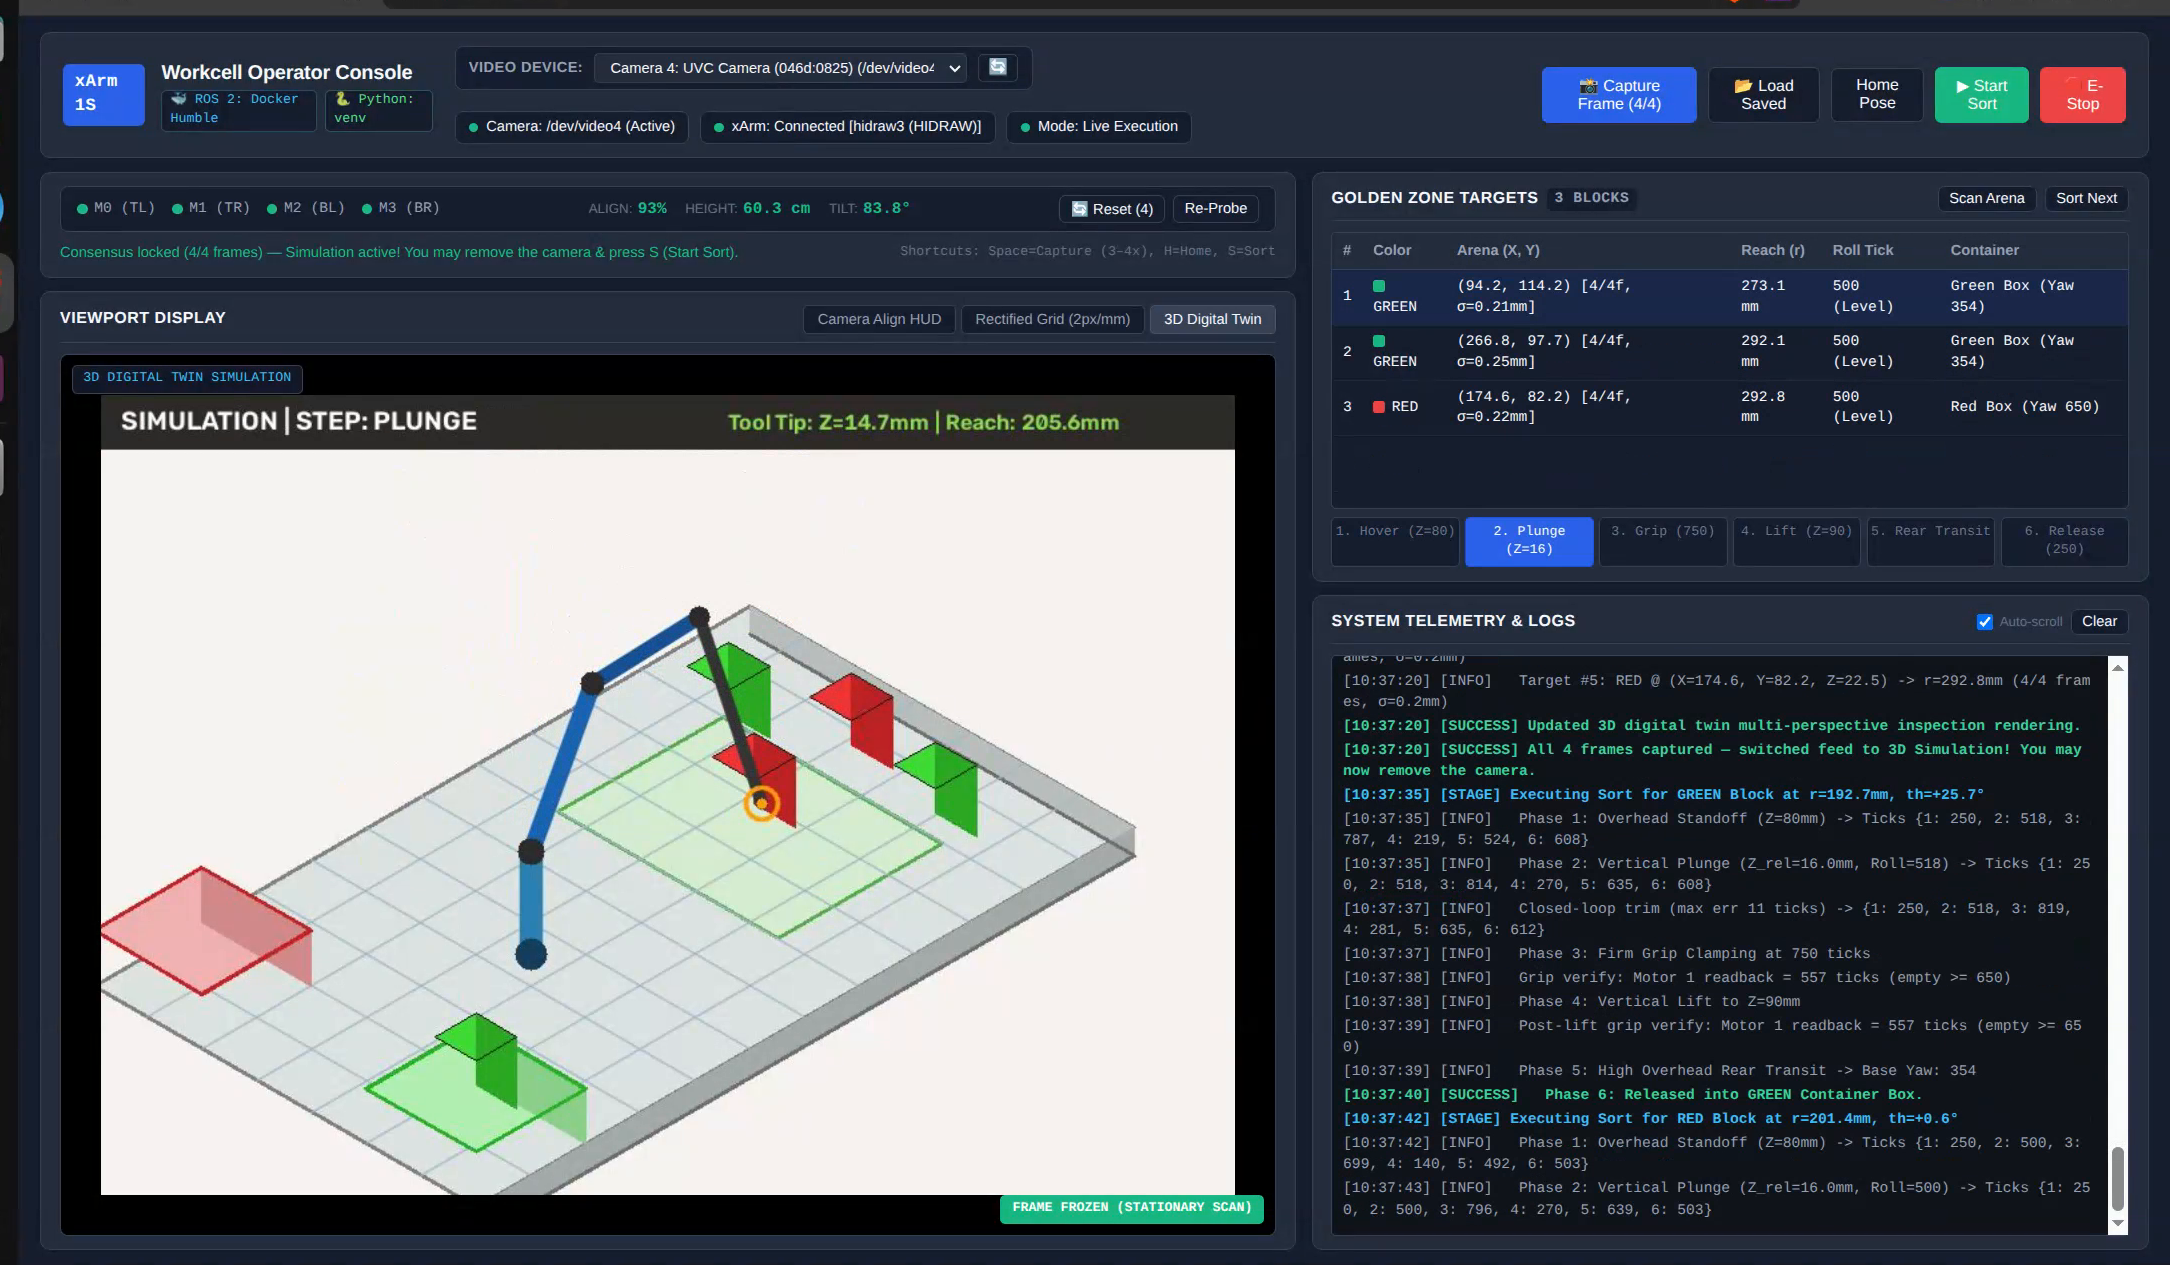
\includegraphics[width=0.96\textwidth]{dashboard_trial1.png}
  \caption{Workcell Operator Console (Web Dashboard) during Trial~1 live execution, showing hardware status, ArUco alignment telemetry, synchronized 3D Digital Twin, Nearest-First queue, and Motor~1 potentiometer logs.}
  \label{fig:dashboard}
\end{figure}

Figure~\ref{fig:trial2_seq} illustrates Trial~2 from the external side camera, showing mid-air overhead transfer of a grasped green block and the final sorted state where green blocks are grouped/stacked on the rear-right zone and red blocks are placed together on the rear-left zone.

\begin{figure}[H]
  \centering
  \begin{subfigure}[b]{0.48\textwidth}
    \centering
    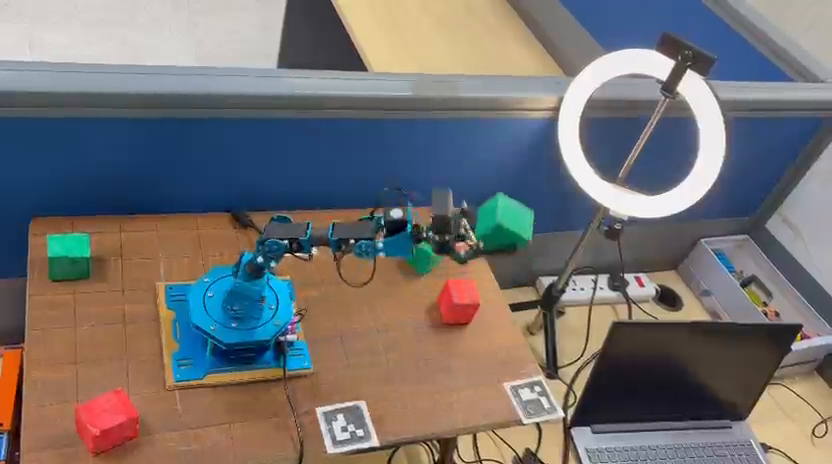
\includegraphics[width=\textwidth]{trial2_midair_flip.png}
    \caption{Mid-air overhead transfer during Cycle~4 after vertical extraction.}
  \end{subfigure}
  \hfill
  \begin{subfigure}[b]{0.48\textwidth}
    \centering
    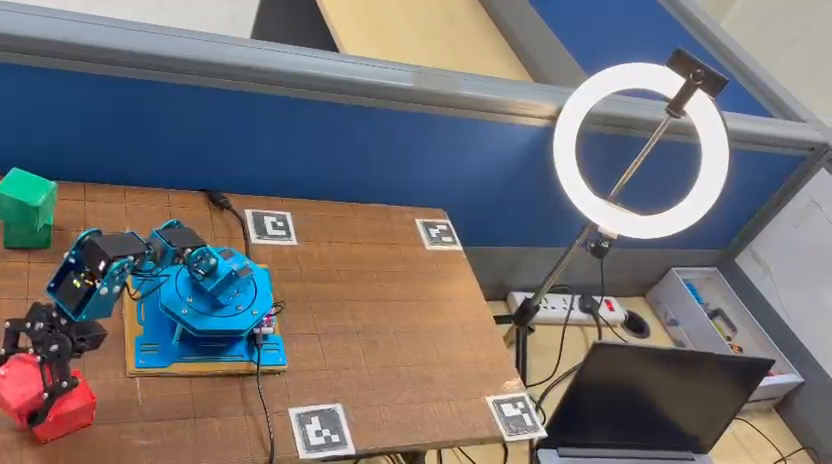
\includegraphics[width=\textwidth]{trial2_final.png}
    \caption{Final sorted state: green blocks stacked/grouped on rear-right, red blocks on rear-left.}
  \end{subfigure}
  \caption{Side-view hardware execution (Trial 2) under 10" LED ring-light illumination.}
  \label{fig:trial2_seq}
\end{figure}

\subsection{Overhead Arena Sequence Analysis (Trial 3)}
To inspect top-down spatial clearance relative to neighboring blocks and the corner ArUco markers, Trial~3 was recorded from an overhead viewpoint ($42.77\text{ s}$ at $28.62\text{ FPS}$). Table~\ref{tab:demo_log} documents the cycle-by-cycle sorting order, and Figure~\ref{fig:demo_seq} presents four sequential stills from the run.

\begin{table}[H]
  \centering
  \small
  \caption{Observed Pick-and-Place Sequence in the 42.8\,s Live Hardware Demonstration}
  \label{tab:demo_log}
  \begin{tabularx}{\textwidth}{@{}c c c l l X@{}}
    \toprule
    \textbf{Cycle} & \textbf{Interval (s)} & \textbf{Color} & \textbf{Initial Location} & \textbf{Destination} & \textbf{Observed Outcome} \\
    \midrule
    1 & $0.0\text{--}7.5$   & Green & Center near-field & Rear-Right (Green) & Clean plunge grasp, overhead rear-flip, placed upright. \\
    2 & $7.5\text{--}15.0$  & Red   & Right mid-field   & Rear-Left (Red)    & Clean grasp and rear-flip placement without disturbing neighbors. \\
    3 & $15.0\text{--}22.5$ & Red   & Left mid-field    & Rear-Left (Red)    & Placed cleanly adjacent to Red block \#1. \\
    4 & $22.5\text{--}32.0$ & Green & Far-right cell    & Rear-Right (Green) & Far reach pick succeeded; placed beside Green block \#1. \\
    5 & $32.0\text{--}41.5$ & Green & Far-center cell   & Rear-Right (Green) & Cleanly cleared final block; 5/5 sorted in $42.8\text{ s}$ ($\approx 8.5\text{ s}$/block). \\
    \bottomrule
  \end{tabularx}
\end{table}

\begin{figure}[H]
  \centering
  \begin{subfigure}[b]{0.235\textwidth}
    \centering
    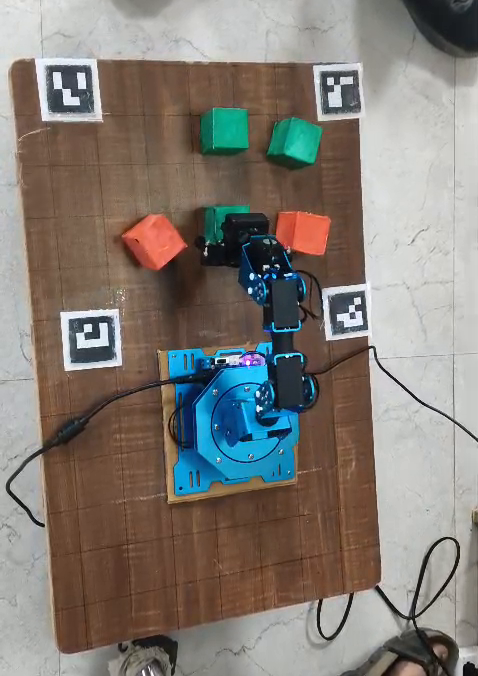
\includegraphics[width=\textwidth]{demo_pick_green1.png}
    \caption{t = 2.0\,s: Near-field pick (Green \#1).}
  \end{subfigure}
  \hfill
  \begin{subfigure}[b]{0.235\textwidth}
    \centering
    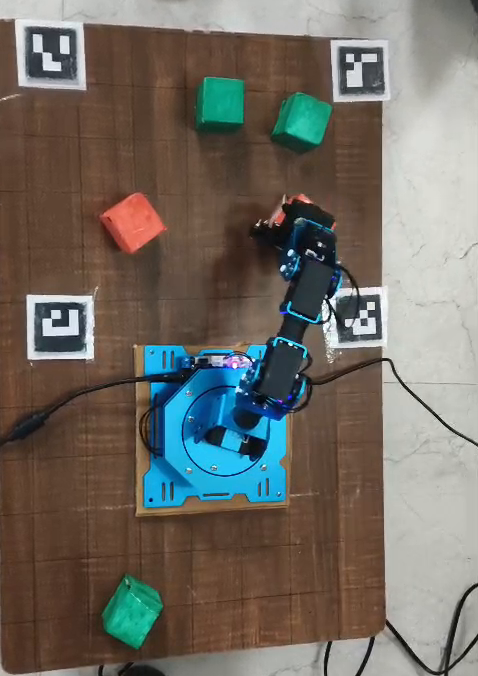
\includegraphics[width=\textwidth]{demo_drop_red1.png}
    \caption{t = 11.2\,s: Green \#1 sorted; picking Red \#1.}
  \end{subfigure}
  \hfill
  \begin{subfigure}[b]{0.235\textwidth}
    \centering
    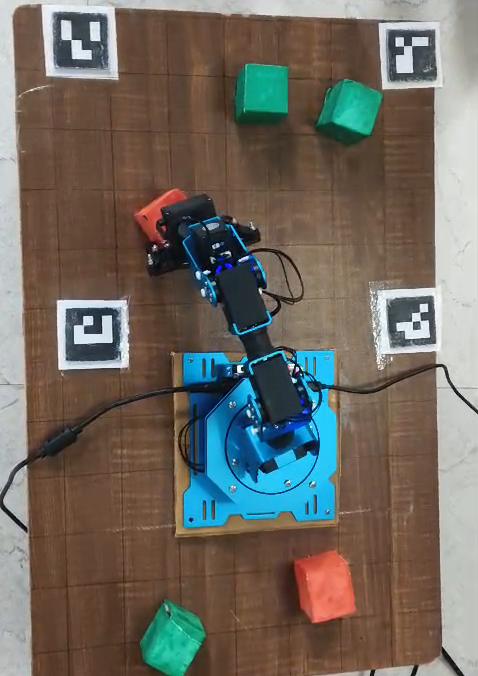
\includegraphics[width=\textwidth]{demo_pick_red2.png}
    \caption{t = 18.0\,s: Red \#1 sorted; picking Red \#2.}
  \end{subfigure}
  \hfill
  \begin{subfigure}[b]{0.235\textwidth}
    \centering
    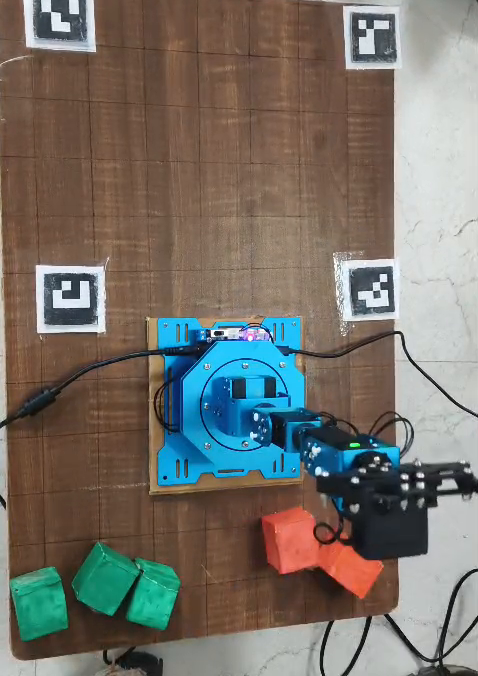
\includegraphics[width=\textwidth]{demo_final_sorted.png}
    \caption{t = 40.5\,s: All 5 blocks cleanly sorted.}
  \end{subfigure}
  \caption{Key frames from the live hardware demonstration video showing Nearest-First picking and overhead rear-flip placement of 3 green and 2 red blocks.}
  \label{fig:demo_seq}
\end{figure}

\subsection{Vision Rectification and Kinematic Reachability}
Figure~\ref{fig:vision_real} presents an actual rectified capture ($600 \times 500\text{ px}$ at $2.0\text{ px/mm}$) from the Logitech C270 camera showing locked corner ArUco markers, the highlighted Central Pickup Zone, and detected red and green blocks annotated with polar coordinates $(r, \theta)$ and wrist roll ticks. Figure~\ref{fig:kin_grid} shows the offline workspace traversal test across 20 central pickup grid points, confirming $20/20$ ($100.0\%$) analytical IK reachability.

\begin{figure}[H]
  \centering
  \begin{subfigure}[b]{0.48\textwidth}
    \centering
    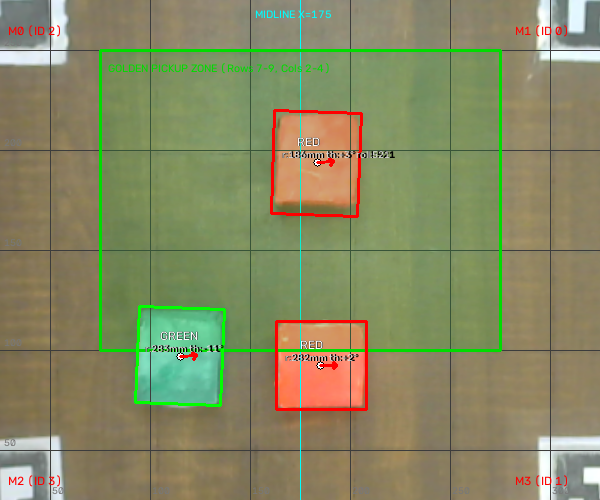
\includegraphics[width=\textwidth]{rectified_arena_detection.png}
    \caption{Rectified $600\times 500\text{ px}$ overhead Logitech C270 capture with polar coordinate overlays.}
    \label{fig:vision_real}
  \end{subfigure}
  \hfill
  \begin{subfigure}[b]{0.48\textwidth}
    \centering
    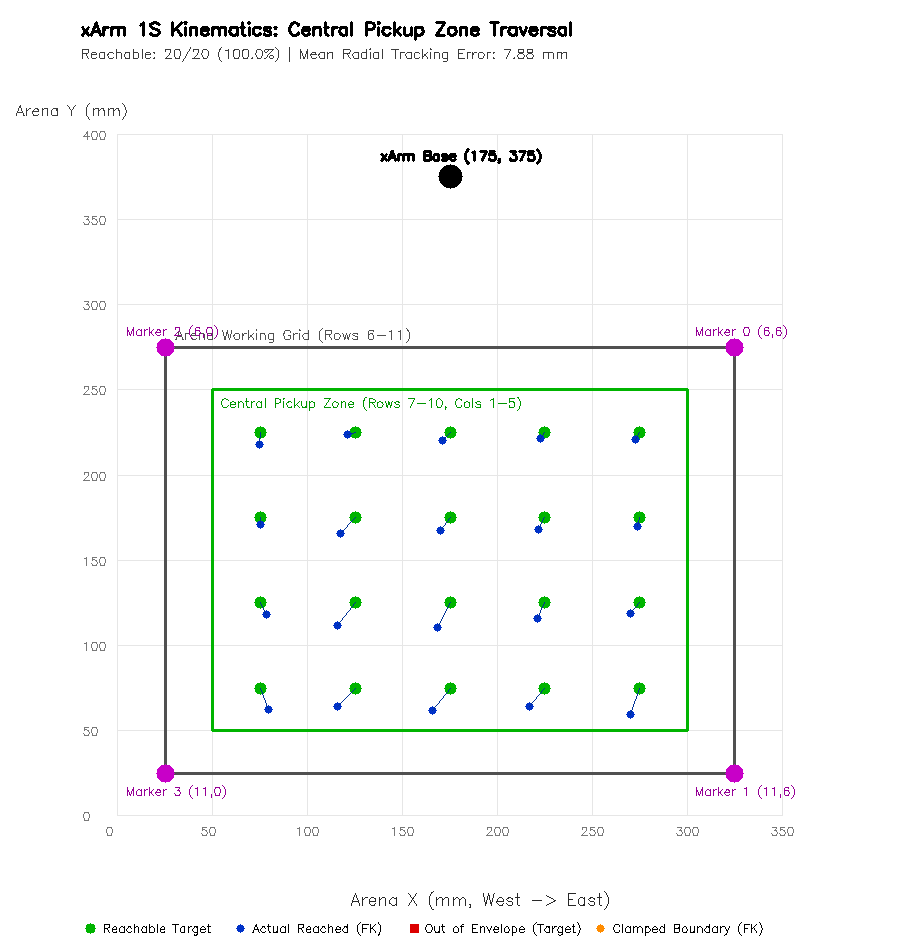
\includegraphics[width=\textwidth]{grid_kinematics_analysis.png}
    \caption{Central pickup zone kinematic traversal confirming $20/20$ ($100.0\%$) reachability.}
    \label{fig:kin_grid}
  \end{subfigure}
  \caption{Experimental vision rectification output and analytical kinematic reachability verification.}
\end{figure}

\subsection{Automated Offline Unit Test Results}
Running the standalone verification suite (\texttt{ros2\_ws/\allowbreak src/\allowbreak sorting\_arm/\allowbreak test/\allowbreak run\_tests.py}) in the project Python virtual environment passed \textbf{43 out of 43 tests} with 0 failures:
\begin{itemize}[noitemsep]
  \item \texttt{test\_calibration\_and\_features} (10/10): atomic YAML persistence, quintic/cubic trajectory scaling, $\pm 25$-tick deviation clamping, HID stale-packet draining, telemetry drift logging, and FK/IK consistency.
  \item \texttt{test\_camera\_alignment} (6/6): projective diagonal intersection, centered and tilted synthetic frame diagnostics, HUD rendering, and alignment JSON output.
  \item \texttt{test\_kinematics} (17/17): reachable envelope checks, out-of-reach rejection, FK/IK roundtrip accuracy, natural pitch safety, distance-scaled sag trim, and rear drop target lookup.
  \item \texttt{test\_vision\_pipeline} (10/10): ArUco homography rectification, red/green HSV segmentation, multi-frame consensus filtering, Nearest-First ordering, proximity-guarded retry limits, and wrist roll alignment.
\end{itemize}

\subsection{Summary of Failure Modes and Mitigations}
\begin{table}[H]
  \centering
  \small
  \caption{Key Failure Modes and Implemented Software/Hardware Mitigations}
  \label{tab:risks}
  \begin{tabularx}{\textwidth}{@{}>{\raggedright\arraybackslash}p{3.5cm} >{\raggedright\arraybackslash}p{3.6cm} X@{}}
    \toprule
    \textbf{Failure Mode} & \textbf{Root Cause} & \textbf{Implemented Mitigation} \\
    \midrule
    Base $240^\circ$ Deadzone & Limited LX-15D servo ROM & Overhead rear-flip restricts Motor~6 to $354\text{--}650\text{ ticks}$ ($71^\circ$ span). \\
    Chassis Self-Detection & Blue anodized aluminum links & Blue HSV band disabled + spatial mask over Rows~3--5, Cols~2--4. \\
    Foreground Block Knocking & Reaching outer blocks over inner ones & Strict Nearest-First ascending radial queue ordering. \\
    Cantilever Droop & Link flex and gearbox backlash & Distance-scaled sag compensation ($r > 185\text{ mm}$) + M2 level lock. \\
    Missed or Slipped Grasp & No tactile fingertip sensors & Closed-loop Motor~1 readback at clamp and post-lift + guarded retry. \\
    Camera Shake / Jitter & Handheld or unfixed overhead camera & 4-frame Snap \& Lock spatial consensus clustering + homography lock. \\
    \bottomrule
  \end{tabularx}
\end{table}

% ============================================================================
% SECTION 6: CONCLUSION & FUTURE WORK
% ============================================================================
\section{Conclusion and Future Work}

\subsection{Conclusion}
The single-arm dual-color sorting system demonstrates reliable autonomous pick-and-place sorting using accessible desktop robotics hardware. Combining coplanar ArUco planar homography, \texttt{solvePnP} parallax correction, multi-frame spatial consensus, analytical polar inverse kinematics with distance-scaled sag compensation, closed-loop Motor~1 potentiometer grasp verification, and an overhead rear-flip transfer motion enables accurate sorting without specialized tactile sensors or industrial actuators. Across three independent live hardware trials, the system achieved 15/15 (100\%) clean pick-and-place sorting with sub-millimeter multi-frame perception repeatability ($\sigma \le 0.37\text{ mm}$), supported by 43/43 passing offline unit tests across all core software modules.

\subsection{Future Work}
Planned extensions include adding 3D-printed V-groove compliant TPU fingertip pads to increase torsional grip stability, integrating an optical break-beam sensor across the gripper jaws for instantaneous contact detection, adding passive shoulder tension springs to reduce Motor~5 static gravity load, and implementing live image-based visual servoing (IBVS) during Phase~1 standoff hover when operating with a permanently mounted overhead camera.

\end{document}
